\chapter{Epithelium}

\section{About Epithelium}
Here I present my implementation of the Honda-Nagai Model for epithelial tissue development as the simulation software called \emph{Epithelium}. The software is easy to install, takes up less than 50Mb, comes in parallel and non-parallel versions (Version 2.0.0, Version 1.0.0) and has very few dependencies. \emph{Epithelium} allows users to specify all parameters of interest in easily modifiable text configuration files, can handle simulations of arbitrarily large size, and can generate data for animations of epithelial tissue development as well as useful plots of important variables. 
\begin{figure}
\centering
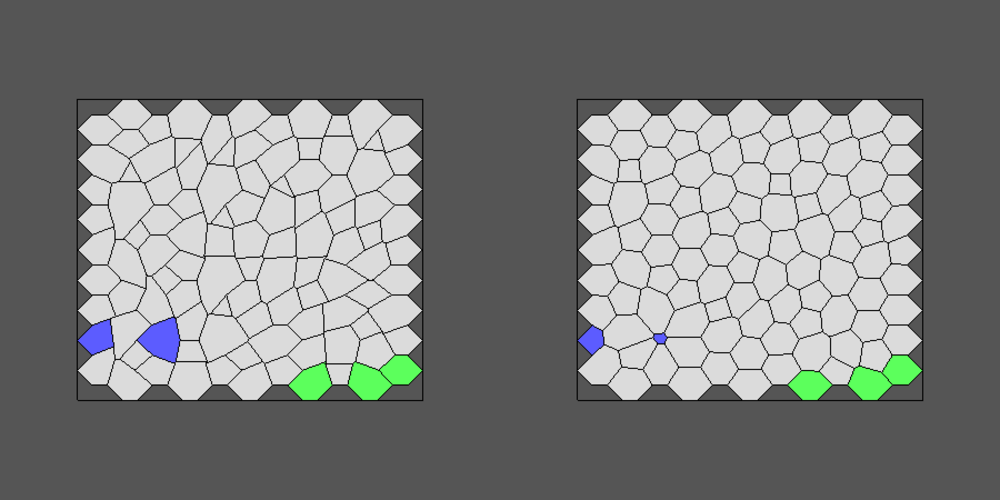
\includegraphics[width=\textwidth]{../diagrams/BeforeAfter.png}
\caption{Cells before (left) and after (right) the application of force.}
\label{fig:beforeafter}
\end{figure}
The source code is highly modularized and allows for ambitious users to easily extend the code to meet their needs. For example, alternate numerical integrators can easily replace the existing one, new mesh generators can replace the square mesh I have developed, and all data is output in space-separated formats which users with scripting language experience can transform to serve as input into the graphical utilities of their choice. In addition, the cell and coordinate classes are well documented and can be extended to output new data, as users may need. Figure~\ref{fig:beforeafter} provides a taste of the what the most basic installation of \emph{Epithelium} can do, showing a mesh of cells before and after equilibration.

\section{Sample Configuration Files}
The typical user will not want to modify source code, but would prefer to have a simple interface for changing simulation parameters. In this section we will explore in depth what the user interface looks like in terms of the three main configuration files, \texttt{config.txt}, \texttt{parameters.txt} and \texttt{change\_mesh.txt}.
\subsection{config.txt}
In this file, the user can specify some global properties about the mesh, and some important quantities for how the simulation will proceed. Most of the quantities are self explanatory. The \texttt{dimension} of the mesh refers to the number of cells along a given axis in a square mesh, and the \texttt{swap length}, \texttt{upper bound}, and \texttt{max swaps} parameters are used for performing random transformations to the mesh in the beginning of the simulation. The \textt{swap length} is the edge length below which a swap is performed. The \texttt{max swaps} parameter is the maximum number of random perturbations the code will make to the mesh before starting the simulation. The \texttt{upper bound} is an integer which is upper bound of the range for a random number generator. A random number generator produces a number in the range [1:\textt{upper bound}], and a random T1 swap is performed on `1'. The \texttt{delta} parameter specifies how close two vertices must be to force a T1 swap to occur.

OFF is the file format given to the plotting program \textbf{geomview} to plot the mesh. You can specify how often the code prints an image with the \texttt{frequency} parameter, but it must be a multiple of ten. More closely spaced images can be generated by using a smaller integration step size.
\begin{lstlisting}
13 # Dimension of mesh MUST BE ODD!!!!
0.01 # Maximum step size
1000 # Number of iterations
10 # frequency of OFF file output. Must be a multiple 10!
.1 # delta minimum vertex separation.
1000 # max swaps
1.5 # swap length
2 # upper bound random number generator
1 # Make energy and shape plots?
1 # Make a movie in the end? [1/0]
\end{lstlisting}

\subsection{parameters.txt}
In the \texttt{parameters.txt} file, the user can specify the parameters discussed in Chapter~\ref{chap:intro}. These are the default parameters for all of the cells in the tissue.
\begin{lstlisting}
beta = 3;
lambda = 55;
t_gamma = 1;
t_area = 4.0;
\end{lstlisting}

\subsection{change\_mesh.txt}
While the parameters file allows global control of the mesh, the \texttt{change\_mesh.txt} file allows users to change local properties of the mesh. The first line of the file is for specifying how many $\gamma$, $A_0$, $\lambda$, and $\beta$ modifications will be made to the mesh. Note that $P_0$ cannot be changed, as $P_0$ is a function of $A_0$ (See Chapter~\ref{chap:intro}). The subsequent lines are for specifying the index and new value for each one of these modifications. As can be seen in Figure~\ref{fig:beforeafter}, cells can be color coded by parameter value to show these changes to the default settings.
\begin{lstlisting}
2 3 1 1 # num gamma, num area, num lambda, num beta
16 4.0  # gamma
17 5.1  # gamma
3 1.0   # area
4 1.0   # area
10 3.7  # area
1 10    # lambda
90 100  # beta
\end{lstlisting}

\section{Image Gallery}
Model parameters are easy to change in \emph{Epithelium}, and a variety of simulations are possible with very minimal effort on part of the user. Figure~\ref{fig:g1} - Figure~\ref{fig:g3} show the output from \emph{Epithelium} for several parameterizations, and can be compared to the output of the original Honda-Nagai model in Figure~\ref{fig:fourgraphs}. Each of the plots show the decreasing energy in the mesh over time, the equilibrium distribution of cell areas, perimeters, and shapes. You may notice that there is very little variation between the plots - this is an essential property of the Honda-Nagai Model~\cite{HondaNagai} that the introduction of cell proliferation and an unbounded mesh could change.  

\begin{figure}
\centering
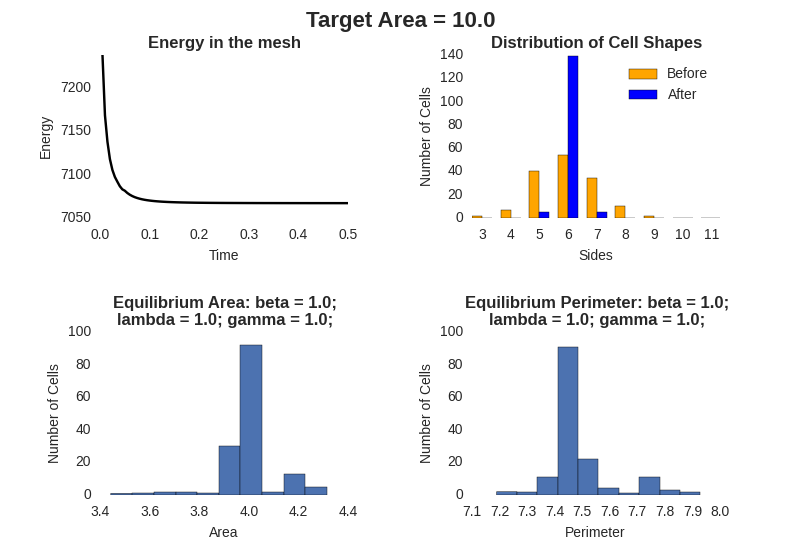
\includegraphics[height=0.4\textheight]{../diagrams/graphs4.png}
\caption[\textbf{Simulation output.}]{\textbf{Simulation output}}
\label{fig:g1}
\end{figure}

\begin{figure}
\centering
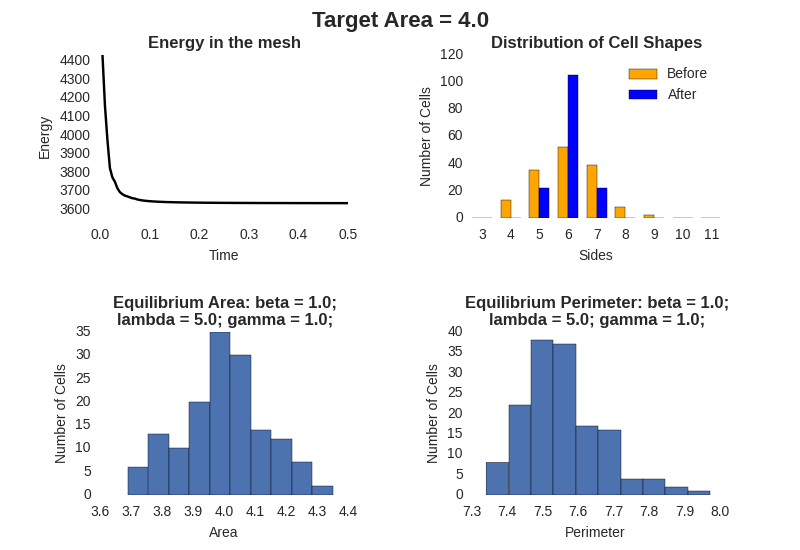
\includegraphics[height=0.4\textheight]{../diagrams/graphs2.png}
\caption{\textbf{Simulation output}}
\label{fig:g2}
\end{figure}

\begin{figure}
\centering
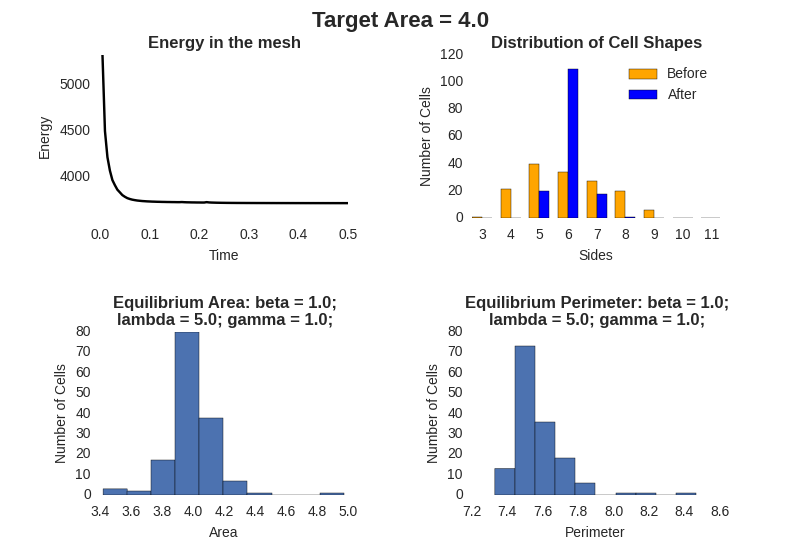
\includegraphics[height=0.4\textheight]{../diagrams/graphs3.png}
\caption{\textbf{Simulation output}}
\label{fig:g3}
\end{figure}

\section{The Design of \emph{Epithelium}}
The technical details of how a vertex dynamics model can be effectively implemented are not explained in great depth in the literature\footnote{\cite{ChasteMain} is an exception, but is rather advanced}. I will fill the void in this field in the section that follows and present a detailed look at the data structures and algorithms needed for the programming of the Honda-Nagai Model. It is fitting to start with a very high-level overview of the structure of the code.

\subsection{[Highly Simplified] Pseudocode}
Here I will briefly outline how the code works. All of the functions are explained in some detail later in this chapter.
\begin{lstlisting}
mesh_variables <- read_configs()
mesh <- make_mesh()
random_alterations(mesh)
copy(mesh, rotate_mesh)
rotate(rotate_mesh)
print(simulation_info) # So the user can verify all parameters.
for i = 1:num_iters
   if(iter%print_freq == 0)
      print(OFF_file)
   temp_mesh = NagaiHondaForce(mesh) 
   temp_rotate_mesh = NagaiHondaForce(rotate_mesh)
   mesh <- mesh + temp_mesh
   rotate_mesh <- rotate_mesh + temp_rotate_mesh
   performT2(mesh)
   performT1(mesh)
   performT2(temp_rotate_mesh)
   performT1(rotate_mesh)
rotate_back(rotate_mesh)
compare_mesh(mesh, rotate_mesh)
print(graphics and error analysis)
\end{lstlisting}

\subsection{Classes}
\emph{Epithelium} has a partially object oriented design. The cell and vertex classes organize the data into meaningful pieces.
\begin{itemize}
\item The {\color{red} Cell} class contains a number of useful functions and data members to make the code easy to read and understand. All cell information could have been stored in arrays, but the OO structure makes the code more readable. All cells know their index, which vertices make them up, they are able to calulate their area and perimeter, can modify their constituent vertices, can tell you whether or not ther contain a vertex, and can print out a graphical, color coded representation of themselves to an OFF file. For information about further functionality of the cell class, the reader is referred to the \texttt{cell.cpp} file in the source code. For information about downloading the source code, see appendix~\ref{appendix}. 
\begin{lstlisting}
public:
 cell(int index, vector<int> AssociatedVertices,\
       double target_area = t_area, double gamma = t_gamma)
 {	
   assert(index >= 0);
   m_AssociatedVertices = AssociatedVertices;
   m_index = index;
   m_target_area = target_area;
   m_target_perimeter = sqrt(pi * m_target_area);
   m_gamma = gamma; 
 }
	
 cell(){} // Default constructor
	
 vector<int>GetVertices(){return m_AssociatedVertices;};
 int GetIndex(){return m_index;};
 void SetIndex(int index){m_index = index;};
 void SetTargetArea(double area){m_target_area = area;};
 double GetTargetArea(){return m_target_area;};
 double GetTargetPerimeter(){return m_target_perimeter;};
 double ComputeArea(double * X, double * Y);
 double ComputePerimeter(double * X, double * Y);
 void PrintCell(ofstream &OffFile);
 int ContainsVertex(int index);
 void SetGamma(double gamma){m_gamma = gamma;};
 double GetGamma(){return m_gamma;};
 void InsertVert(int v1, int v2);
 void EraseVert(int index)
 {
   vector<int>::iterator it = find(m_AssociatedVertices, index); 
   m_AssociatedVertices.erase(it);
 };
 void ReplaceVert(int before, int after)
 {
   vector<int>::iterator it = find(m_AssociatedVertices, before); 
   *it = after;
 };
 void SetVertices(vector<int> vertices)
 {
   m_AssociatedVertices = vertices;
 };
 int GetNumSides(){return m_AssociatedVertices.size();};
private:
 vector<int> m_AssociatedVertices; // Stored counterclockwise
 int m_index;	
 double m_target_area;
 double m_target_perimeter;
 double m_gamma;
};

\end{lstlisting}

\item The {\color{green} Vertex} class stores the index of a vertex, and 
whether or not the vertex will move during the integration. While a 
vertex object does not store the location of the vertex, it tells the 
simulator whether or not a vertex is on the border of a mesh and, if it 
is not, it is allowed to move. It was a design choice that 
\emph{Epithelium} be able to run three popular types of meshes, those 
with border, those without, and those that cover a surface.  Another 
benefit of the vertex class is that is allows users to easily extend 
the code to include forces acting on individual vertices, and to 
specify other types of vertices besides interior and exterior. The 
vertex class could be extended to include a member function such as 
activeMigration(), or any number of interesting functions. This code was developed with eyes to the future. 
\begin{lstlisting}
class vertex
{
public:
  vertex(int idx, bool t) : index(idx), IsInner(t){};
  vertex(){index = -1; IsInner = 0;};
  int index;
  bool IsInner;
  inline bool operator==(const vertex& rhs)
  {return index == rhs.index;};
};
\end{lstlisting}
\end{itemize}


\section{A Relational Database}
There is one other major idea behind the design of \emph{Epithelium}. A 
popular way to store data since the 1970's is to store data in groups of tables which are connected via \emph{keys}. This type of database is popular for reasons which will become apparent by means of a simple example. 

Consider a business which sells a number of products, and wants to keep 
track of their customers, the customer's orders, the customer's 
addresses, and information about the products ordered. A wasteful way 
to store this data is to create a large table in which the first column 
is for customer names. Next to every customer's name is the customer's 
address, and next to the customers address is the customer's order 
number. Next to the customer's order number is an item in that order, 
and next to each item ordered is the item information. This method of 
storing data is terribly redundant, because for each order with more 
than one item you would have the unnecessary storage of the orderid, and of all 
the customer information. Consider Figure~\ref{fig:rdb}(a.) for an illustration of the concept.
A better idea is to break this data up into several tables which 
together define a \emph{schema}. By defining an appropriate schema, we can minimize the redundancy of information, and extract specific subsets of data in a cache-efficient way. Consider Figure~\ref{fig:rdb}(b.) for an illustration of the concept.

\begin{figure}[h]
\centering
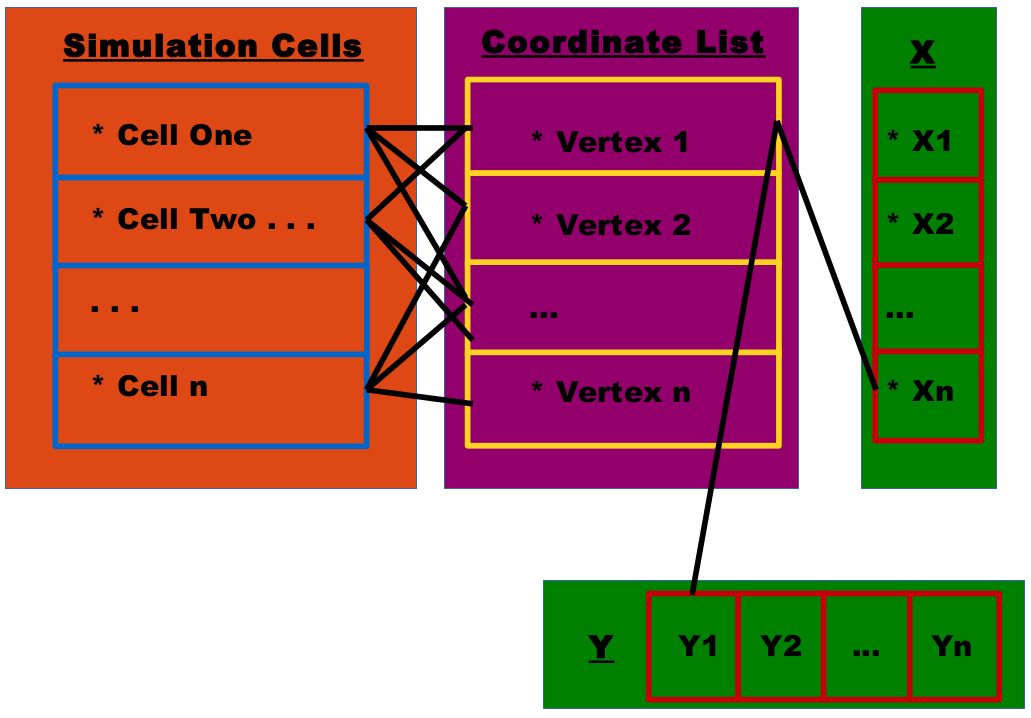
\includegraphics[width=0.5\textwidth]{../diagrams/ds.png}
\caption{\textbf{The Relational Database.}}
\end{figure}

The \emph{Epithelium} datastructure is a schema made up of the simulationCells, vertexList, X, Y, tempX and tempY tables. The cell and vertex tables are implemented as 1d \texttt{std::vectors} of cell and vertex indices, whereas the position tables are implemented as low-level 1d arrays for ease of passing these structures to CUDA C functions. The cells can extract coordinate information from the vertexList table via the \emph{index} key, and the coordinateList can access the position information from the X and Y arrays via their own \emph{index}. The temporary X and Y arrays store temporary position information about the vertices before the mesh positions are updated. This choice saves both memory and time because no data is stored redundantly (e.g. The coordinate information of a vertex is not stored in every cell that contains it) and huge data structures do not need to be passed around when only a small portion of data is required (e.g. When updating vector locations, only the position and temporary positions are passed to a function instead of the entire mesh). 

\section{Initial Mesh Design}
The hex\_mesh() function generates an $n$x$n$ mesh of cells, where the 
dimension represents the number of cells touching the boundary in 
either axial direction. Figure ~\ref{fig:mesh} shows the default mesh 
used by \emph{Epithelium}, with the cell ids and vertex indices labelled. After a sheet of cells is generated by 
hex\_mesh(), the tissue is perturbed by performing random 
T1 swaps on edges of the mesh, and then by perturbing the locations of a select 
number of vertices.

\begin{figure}
\centering
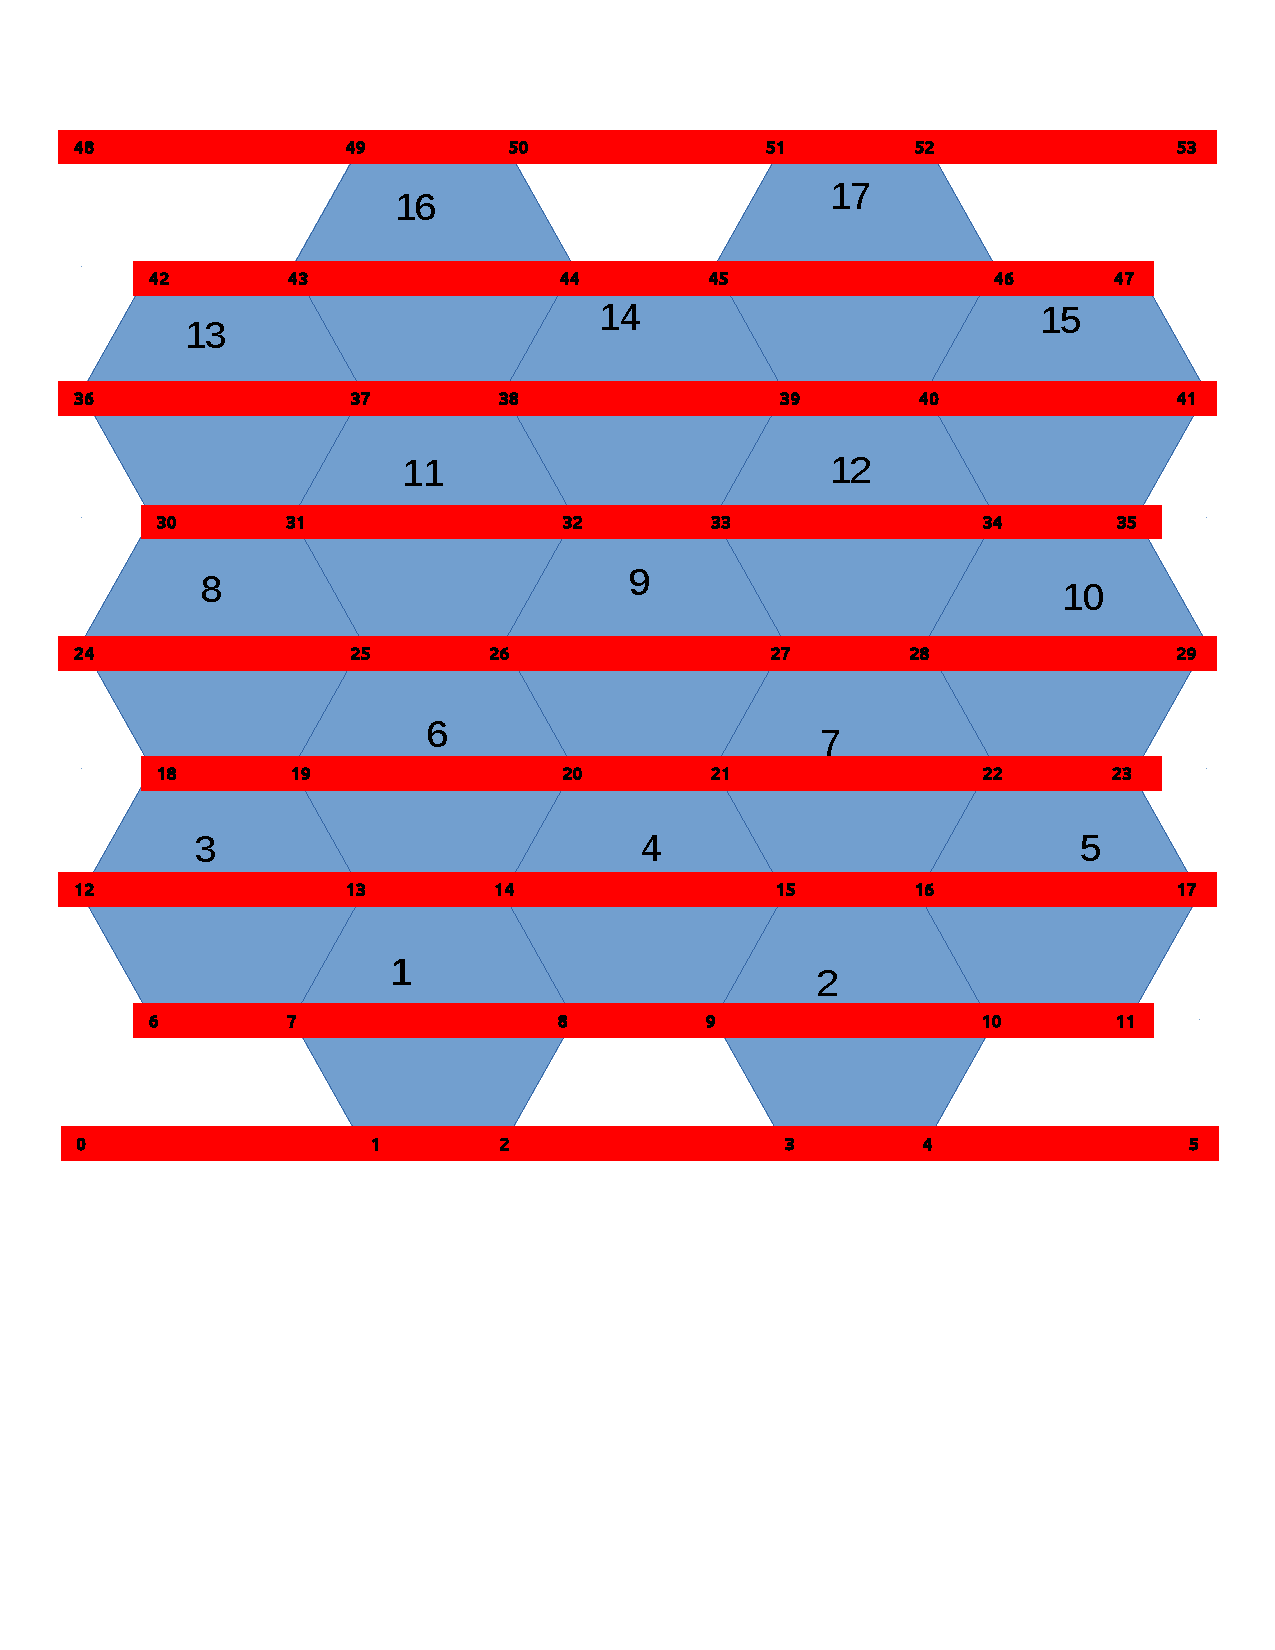
\includegraphics[height=0.7\textheight]{../diagrams/vert_mesh.pdf}
\caption[A 5x5 Hexagonal Mesh.]{\textbf{A 5x5 hexagonal mesh. The cell 
indices are written in the cells and the vertex indices are written on the red bars.}}
\label{fig:mesh}
\end{figure}
\section{Moving the Vertices}
While the data structures behind \emph{Epithelium} are important to understand, the most fundamental idea behind a vertex dynamics model is how the vertices in a tissue are moved.  \emph{Epithelium} transforms the tissue by looping over all of the vertices, computing the force acting on each vertex, and then computing a displacement with the forward Euler method. In their original paper, H. Honda and T. Nagai described the use of a Modified Runge Kutta Method\cite{HondaNagai} to move the vertices, but this method would result in vastly more computations per each time step. The same decision to use then Euler Method was made by the research group at Oxford that developed CHASTE, as well as by the Weliky-Oster team ~\cite{WO}, and so we accept it as a reasonable design decision. 

A displacement is calculated and stored in the temporary X and Y arrays. No vertex is permitted to move more than one half of the minimum delta separating vertices (the $\delta$ under which a T1 swap will occur) during an integration. By imposing this restiction we are ensuring that we will not miss the event of two vertices coming critcally close and a T1 swap occurring. Also, this prevents vertices from passing each other and invalidating the mesh. To ensure that no vertex moves too much, we verify each displacement as we put it in the temporary X and Y arrays. If a displacement is too large, then the entire array of temporary displacements is erased, the time step is halved, and we begin the integration again. For this reason, we could label the integrator as `fault tolerant'.

\begin{wrapfigure}{L}{0.4\textwidth}
\begin{center}
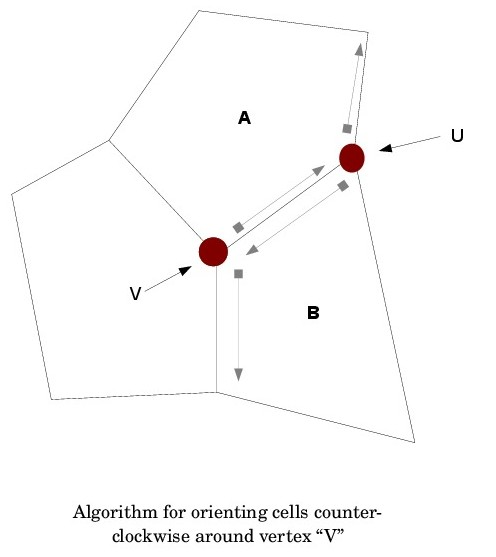
\includegraphics[width=0.38\textwidth]{../diagrams/counterclockwise.jpg}
\end{center}
\caption{Getting Cells in Order}
\label{fig:ctrclockwise}
\end{wrapfigure}

Another important aspect of the numerical integration is that cell and vertex information must be processed in counterclockwise order. When we are integrating a vertex $i$, \mph{Epithelium} first searches in the \texttt{simulationCells} vector for a cell which contains $i$, and then the finds the next vertex $ip1$ in that cell's \texttt{m\_AssociatedVertices}. This step gives us an oriented edge. Some other cell contains that edge if it contains both of the vertices, and, if that cell exists, it must be clockwise from the first (See Figure~\ref{fig:ctrclockwise}). The cells are stored in the reverse order of which they are uncovered by this algorithm before the integration of the equation of motion for $i$ starts. This is a very expensive step ($O(n^3)$) in the computation, and ought to be optimized.

\begin{figure}[hr]
\centering
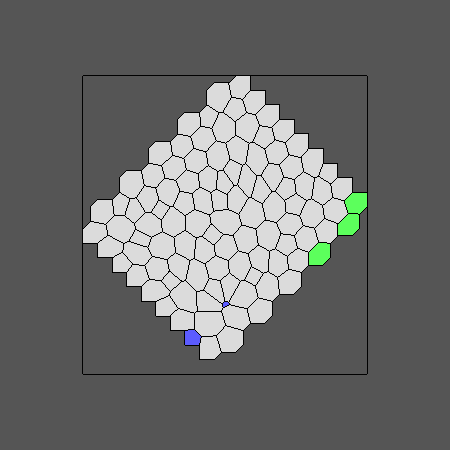
\includegraphics[width=0.5\textwidth]{../diagrams/rotate.png}
\caption{\textbf{A Rotated Mesh for Error Analysis.}}
\label{fig:rotate}
\end{figure}

\section{Error Tolerance of the Algorithm}
\emph{Epithelium} outputs an error measurement at the end of a simulation to give the user a sense of the numerical stability of the code. \emph{Epithelium} runs two simulations at the same time, one on the mesh made by hex\_mesh(), and another on the same mesh which has been rotated 45 degrees (See Figure~\ref{fig:rotate}). In this way, we hope to expose any dynamics which are dependent on the rounding of floating point numbers. Then, at the end of a simulation, the rotated mesh is rotated back and corresponding vertices are compared by index using the Euclidean norm. In practice we see near $\epsilon_{mach}$ error for every simulation.

\section{Embarassing Parallelism and CUDA}
The numerical integrations and the vertex location updates exhibit what Cleve Moler describes as ``embarassing parallelism''. Computing the displacement of vertex \emph{a} does not depend upon the computation of the displacement of vertex \emph{b} during a given time step. Similarly, the vertex locations can all be updated in parallel since the update is simply a vector sum operation of the X and Y arrays with the temporary X and Y arrays, respectively. \emph{Epithelium} employs several parallel routines for these types of operations when it is possible. 

A popular hardware choice for parallel programming in last decade has been the NVIDIA GPU, and an extension of the C language called CUDA was developed to allow programmers to send certain portions of C code the GPU for processing. The GPU is a collection of small processors with very little shared memory, and is well suited so simple computations that can be performed on memory stored in adjacent locations in C arrays. The demand that memory be coalesced has been the single impeding factor in the full CUDA parallelization of \emph{Epithelium}, for while the numerical integrations are \emph{theoretically} parallelizable, data from several arrays (See Section~\ref{sec:rdb}) is used in calculating the force on a vertex.

Nevertheless, CUDA was employed for two obvious parallel tasks, and for one slightly sophisticated one. The sum of the position arrays and the temporary position arrays was done with a simple vector sum, and the rotation of the mesh for error detection was performed by multiplying the coordinates of each vertex in the mesh by the rotation matrix:
\[ \left( \begin{array}{cc}
\cos\theta & -\sin\theta \\
\sin\theta & \cos\theta 
\end{array} \right)\] 
CUDA was employed for the slightly challenging task of calculating the error between the non-rotated and rotated meshes by first subtracting the position arrays of the rotated mesh from the position arrays of the non-rotated mesh. The calculated differences are then stored in $dX$ and $dY$. Next, the pythagorean theorem is used to calculate the distances between the coordinates, and these lengths are stored in the $dist$ array. The maximum distance is then extracted from this array in $log(N)$ time by comparing neighboring elements and discarding the smaller one until only one element remains, giving the maximum $||*||_2$ error in the mesh.

\section{Computing Topological changes.}
Now that we have covered the way that the equation of motion is integrated, we move on to how the topological changes are implemented in \emph{Epithelium}.  

\subsection{The implementation of the T2 swap.}
The PerformT2s() function looks at every triangular cell in the mesh and checks the edge lengths. If the cell has a critically small edge, then the cell is deleted from the mesh. The centroid of the cell is calculated, and this becomes the vertex representing the collapsed triangle. Then, one of the three constituent vertices has its position updated to the centroid coordinate and any cell which previously bordered the triangular element has both vertices related to the triangle deleted from \texttt{m\_AssociatedVertices}. Next, the centroidal vertex is inserted in the position of the deleted vertices. The PerformT2s() function must be called before the PerformT1s() function to make sure that all offending triangular elements are deleted before we perform the T1 swaps, because these cannot be performed on triangular cells. The T1 swap requires four vertices to be performed correctly, as explained in the next section.

\subsection{The T1 Swap}
The PerformT1s() function loops over all of the cells in the mesh, and checks the edge lengths in each cell. If an edge is critically small (less than $\delta$), then a T1 swap must occur. The first step taken by the PerformT1s() function is to find all of the cells and vertices involved in the swap.

Since the critically small edge was detected by looping over all the cells in the mesh and checking their edges, we can identify the cell that initiated the swap (let's refer to is as $c1$). There is another cell in the mesh which contains the offending edge, and we can call that cell $c2$. Since $c1$ contains at least four vertices, then we can label the four vertices of interest, $im1$, $i$, $ip1$, $ip2$. $i$ and $ip1$ are the vertices bounding the small edge, $im1$ is the vertex before $i$, and $ip2$ is the vertex coming after $ip1$. 

Given these indices for the vertices, we can find the other cell in the mesh which contains $ip1$ and $ip2$, which we call $c3$. Finally, we locate the cell containing $im1$ and $i$, and call this cell $c4$. Now that all of the cells are located, we proceed to perform the T1 operation during the course of which $c1$ and $c2$ will cease to be neighbors and $c3$ and $c4$ will become neighbors. 

The midpoint $mp$ of the edge ($i$, $ip1$) is calculated and a perpendicular bisector $b$ is drawn through it. Then centroid ($CN1$) of $c1$ is calculated and the vector pointing from $m$ to $CN1$ defines the direction in which a new vertex should be placed. Next, the centroid ($CN2$) of $c2$ is calculated, and the vector pointing from the $m$ to $CN2$ defines the direction in which the other new vertex should go. This could have been implemented in several ways, but in \emph{Epithelium} $ip1$ is deleted from $c2$ and placed along $b$ in the direction indicated by $CN1$ at a distance of $\delta$ from the midpoint. $i$ is deleted from $c1$ and is moved a distance $\delta$ along $b$ in the direction indicated by $CN2$.

Before the function ends, $i$ is inserted after $ip1$ in $c3$ and $ip1$ is inserted after $i$ in $c4$. Figure ~\ref{fig:t1pdf} offers a visual aid to understanding the swap. The entire operation is easy to implement thanks to the counterclockwise storage of vertices.

\begin{figure}
\centering
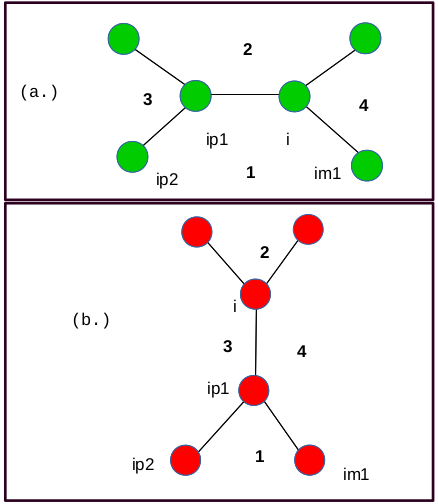
\includegraphics[height=0.5\textheight, keepaspectratio]{../diagrams/t1pdf.png}
\caption[\textbf{Implementation of a T1 swap.}]{\textbf{The implementation of a T1 swap.}}
\label{fig:t1pdf}
\end{figure}
